\documentclass[11pt]{article}
\usepackage{geometry}
\geometry{a4paper}
\usepackage{graphicx}
\usepackage{listings}
\usepackage{booktabs}
\usepackage{amsmath}
\usepackage{epstopdf}
\usepackage{url}
\usepackage[english]{babel}
\usepackage{csquotes}

\usepackage[backend=biber]{biblatex}
\addbibresource{abibfile.bib}

\title{An embedded system, from software to hardware\\\small{(EDAN15 VT15 Final Report)}}
\author{
Anton Eliasson, \texttt{dat11ael@student.lu.se}\\
Daniel Lundell, \texttt{ada10dlu@student.lu.se}
}
%\date{}                                           % Activate to display a given date or no date

\begin{document}
\lstset{
	language=C,
	captionpos=b,
	basicstyle=\footnotesize\ttfamily
}

\maketitle

\begin{abstract}
This report details the laboratory work where, during five sessions, software and hardware solvers of the Greatest Common Divisor were implemented and compared. A software solution was developed for a uniprocessor system and later parallelized to run on a dual processor system. Parts of it were then implemented in hardware. The solutions were profiled and discussed from three perspectives: performance, hardware utilization and energy consumption. The results demonstrate that significant performance improvements and decreased energy consumption can be gained when algorithm implementations approach hardware. It was shown that power and energy consumption do not neccessarily correlate and that an implementation with slightly higher power requirements can have a much lower total energy consumption.
\end{abstract}

\section{Introduction}
This is a report on the laboratory work in the \emph{Design of Embedded Systems (EDAN15)} course at LTH. The purpose of the laboratories is to use and implement an embedded system and to observe how different implementations differ in relation to effiency, power and hardware utilization. The assignment is first solved with a pure software solution which is later parallelized and then transformed into a hardware accelerated solution. In addtion the purpose is to explore frameworks and tool chains used in development of embedded systems. The embedded system used in the laboratory is a Xilinx FPGA platform.

The report is organized as follows. Chapter~\ref{sec:exp} describes the experiments conducted throughout the five laboratory sessions. Chapter~\ref{sec:measurements} presents and discusses the measurements obtained during the experiments. Chapter~\ref{sec:summary} concludes the report with a summary.

\section{Experiments\label{sec:exp}}
The experiments were carried out over five lab sessions. The goal was to evaluate software and hardware solutions running on a Xilinix Digilent Nexys-3 FPGA platform. All software was developed in C for the MicroBlaze\cite{microblaze} CPU architecture. The MicroBlaze is very customizable but in this project, the default settings were used. This optimized the CPU for the smallest area. 32 KiB of RAM was assigned to each processor core an AXI bus was used for communication between the CPUs and their peripherals.

The system clock was set to 100 MHz. For timing measurements, an \emph{axi\_timer}\cite{axi-timer} connected to the AXI bus was used. A simple UART, also connected to the AXI bus, was used for communication with the operator. The hardware was described and synthesized using Xilinx Design Suite 14.2. In every solution the performance (run-time), FPGA area utilization and power was recorded for later comparison.

The first laboratory was to implement and compare two pure software solution of a Greatest Common Divisor (GCD) algorithm for N numbers. Furthermore, the software has to run on a single processor system.

The second laboratory session was to implement and evaluate again a pure software solution of a GCD algorithm for N numbers. This time the architecture should use a multi-processor system. The system uses two MicroBlaze processors, working on the same data set.

The third and fourth laboratory session was to select a part of the GCD algorithm for N numbers and implement it in hardware. The hardware core is first written in VHDL and simulated using Xilinx ISE. It communicates with the processor using a Fast Simplex Link interface\cite{fsl}.

The last laboratory session was to integrate the hardware developed in the previous sessions into a larger system. It has software to communicate with the operator over a serial link, similar to the uniprocessor solution, but uses the hardware core for the actual computations.

\subsection{Software algorithms}
The algorithm chosen for computation of the greatest common divisor is the Euclidean algorithm. This was chosen because it is both simple to implement, and because it, in its simplified form that is only valid for positive integers, avoids mathematical operations that are difficult to implement in hardware such as division and modulo. An algoritm in pseudocode to calculate the GCD for two integers\cite[pp. 318-320]{knuth} is shown in listing~\ref{lst:gcd}. To calculate the GCD for an arbitrary number of integers, the fact that the GCD is an associative function is used, so for every $a$, $b$ and $c$, $gcd(a, gcd(b, c)) = gcd(gcd(a, b), c)$ holds.

\begin{lstlisting}[float=tbh,frame=tb,captionpos=b,caption={Euclidean subtracion algorithm},label=lst:gcd]
function gcd(a,b)
	while b != 0 {
		if a > b
			a = a - b
		else
			b = b - a
	}
	return a
}
\end{lstlisting}

\subsection{Single processor}
The single processor system was implemented using a single MicroBlaze core. A simple software program reads data from the serial port, calculate the GCD and outputs it to the user. The GCD used is the one described above.

\subsection{Dual processor}
The dual processor system was implemented using two identical MicroBlaze cores with separate memory. The two cores communicates using two unidirectional Fast Simplex Links (FSL), creating a bidirectional interface. A master-slave model of communication between the cores was used. The master core receives data from the serial link, splits the data set into two halves and sends one half over FSL to the slave core. The cores calculate the GCD for their own halves separately and in the end the slave sends its result back over FSL. The master computes the GCD for the final two values and sends the result back over the serial link.

\subsection{Hardware accelerated}
The part chosen for hardware acceleration was the GCD algorithm for two numbers. The hardware runs on a custom IP core on the same board as the MicroBlaze core running the software. The software reads the input over serial and outputs each element in the data set over FSL to the hardware core. The GCD is computed in hardware and sent back to the MicroBlaze core over FSL.

\begin{figure}
  \centering
  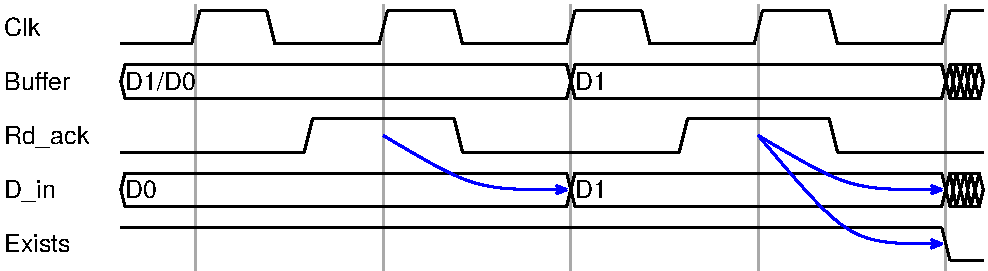
\includegraphics[width=1\textwidth]{timingdiagrams/read.pdf}
  \caption{Timing diagram for an FSL read operation}
  \label{fig:fsl-read}
\end{figure}

Figure~\ref{fig:fsl-write} shows the timing diagram for an FSL read operation. Pulsing the \emph{Rd\_ack} high for one clock cycle causes the next word in the buffer to be moved to \emph{D\_in} on the next low-high clock transition. \emph{Exists} tells the recipient that more data is available in the buffer.

\begin{figure}
   \centering
   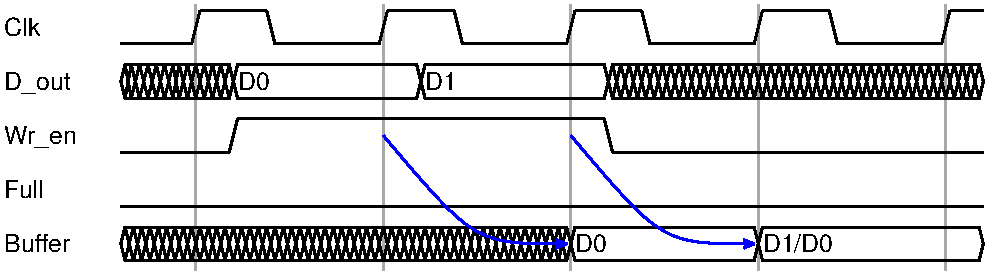
\includegraphics[width=1\textwidth]{timingdiagrams/write.pdf}
   \caption{Timing diagram for an FSL write operation}
   \label{fig:fsl-write}
\end{figure}

Figure~\ref{fig:fsl-write} shows the timing diagram for an FSL write operation. There is no acknowledgement signal here. The sender tells the FSL bus that it is writing a word to \emph{D\_out} on each clock cycle as long as it is holding \emph{Wr\_en} high. It is allowed to do so as long as the recipients buffer is not full, as indicated by the \emph{Full} signal.

\begin{figure}
  \centering
  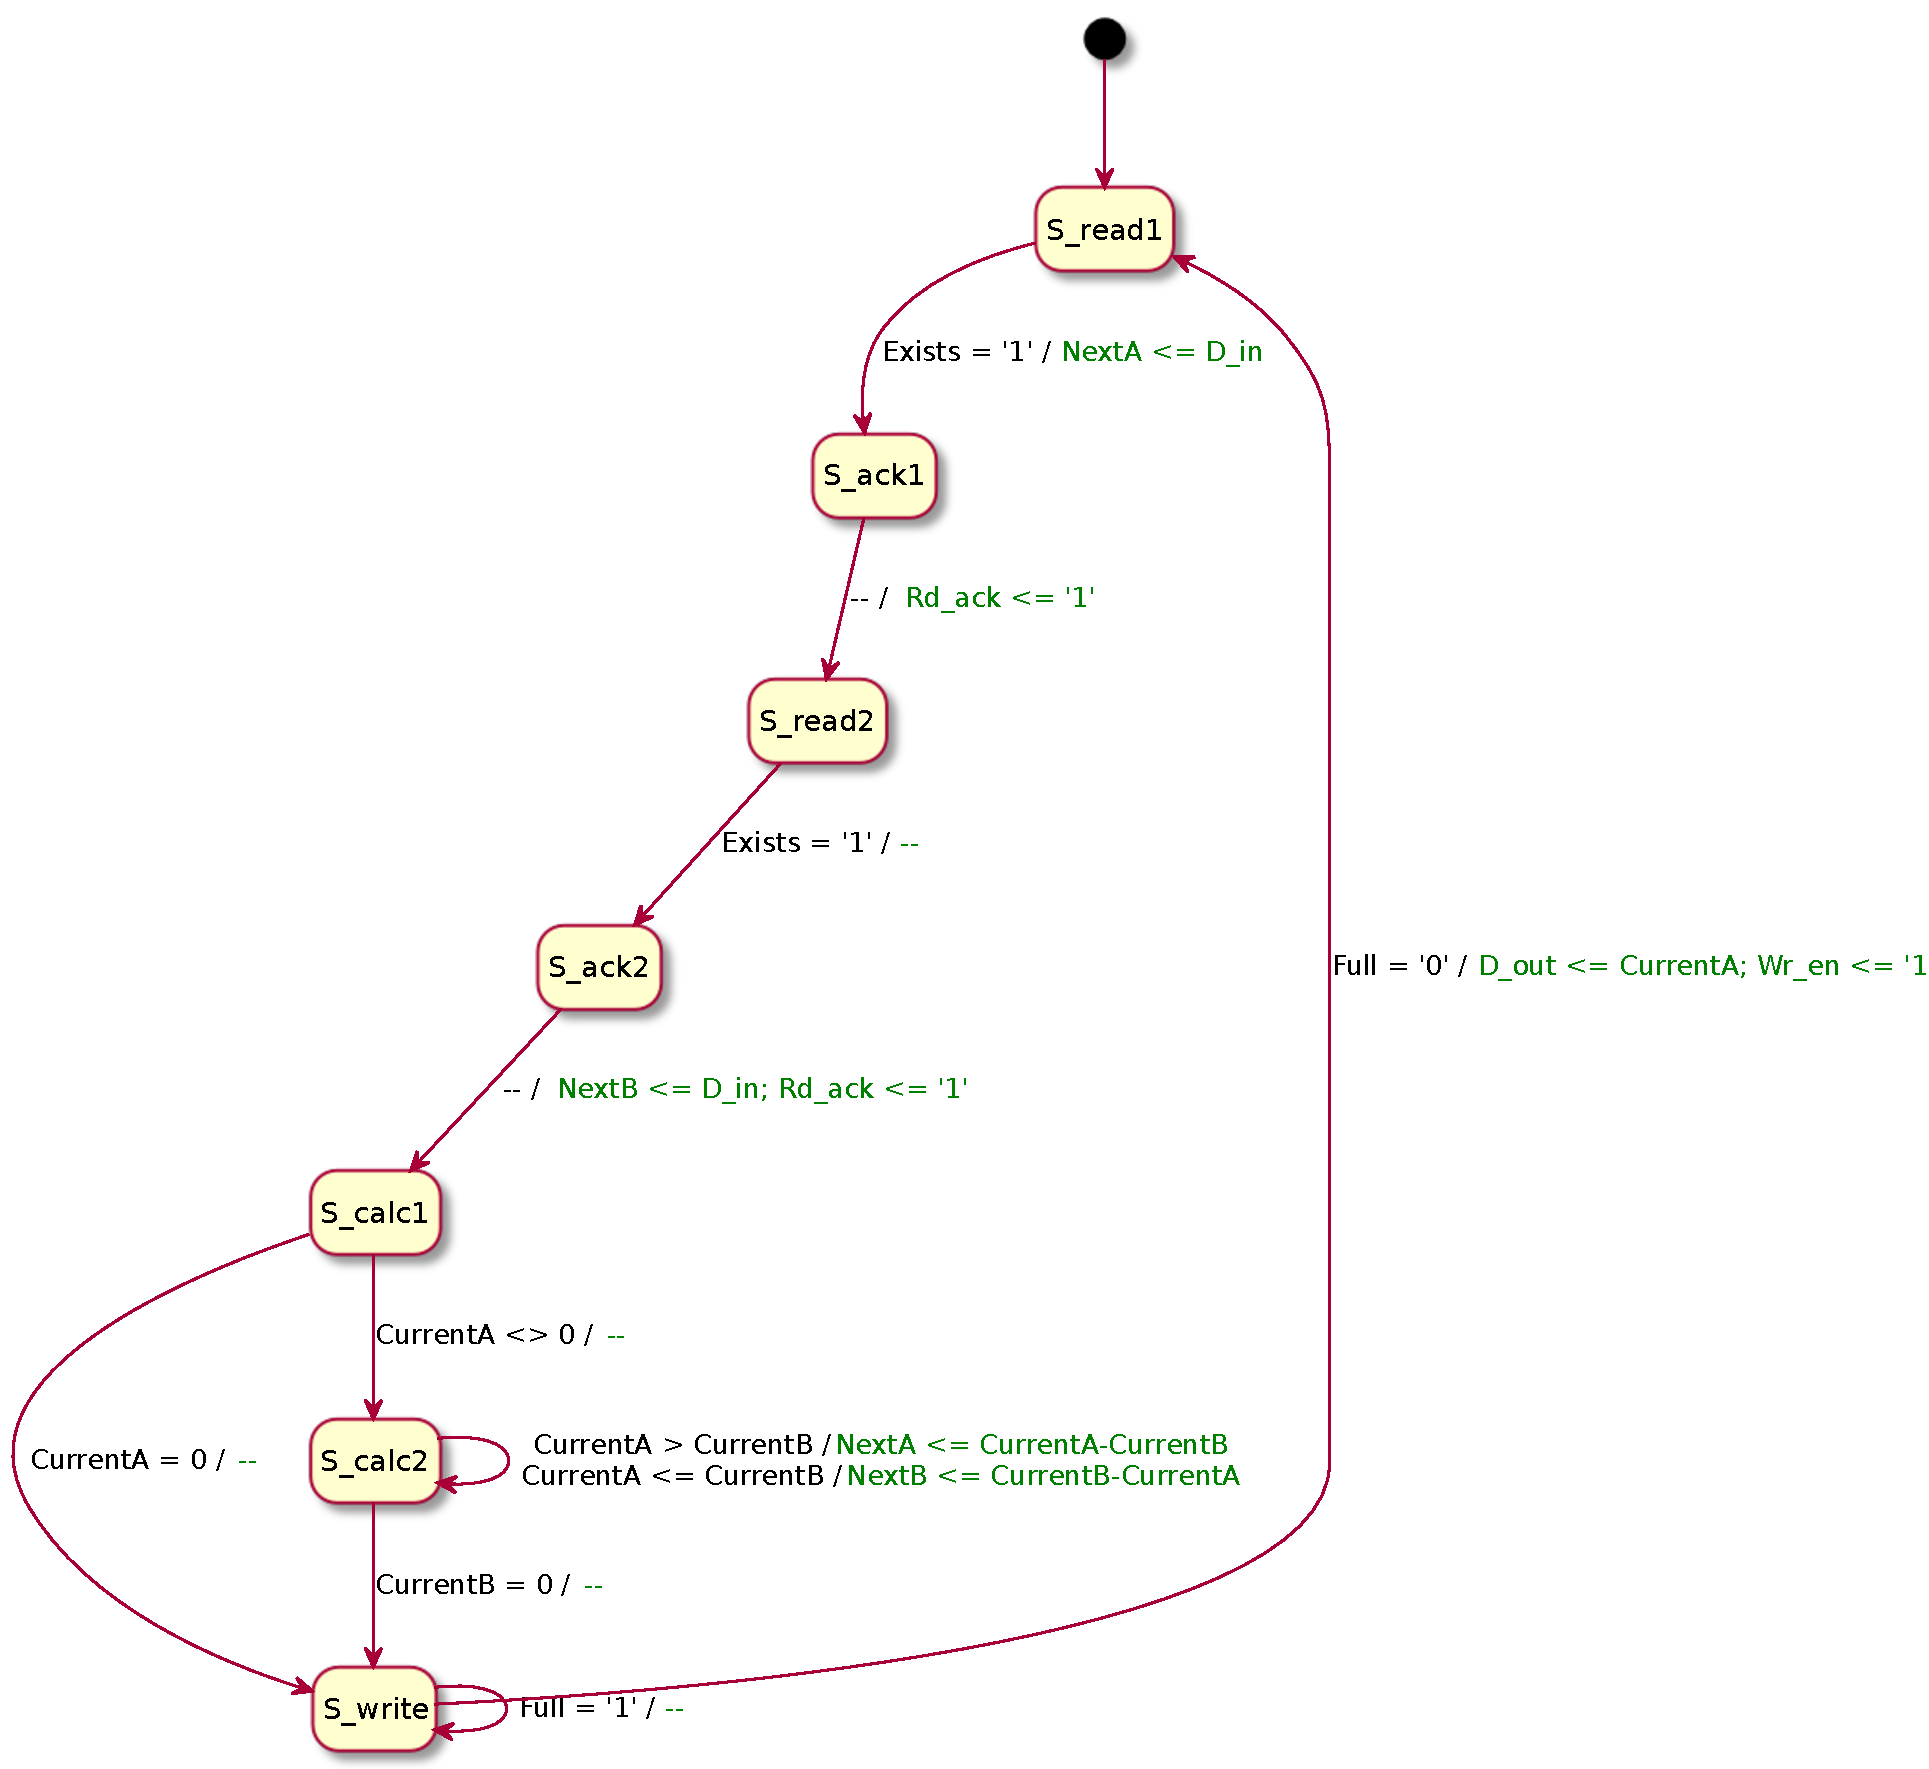
\includegraphics[width=1\textwidth]{statediagrams/hwstatediagram.pdf}
  \caption{State diagram for the custom IP core}
  \label{fig:state}
\end{figure}

A Mealy machine state diagram for the custom IP core is shown in figure~\ref{fig:state}. Inputs are shown in black and outputs in green. Some transitions don't have transition conditions, and some lacks outputs. This is because the state diagram shows a clocked circuit and during some transitions signals like \emph{Rd\_ack} must be held high for exactly one clock cycle and then pulled low again.

\section{Measurements and Discussion\label{sec:measurements}}
This section describes the results obtained from the experiments. To get consistent results, the \emph{axi\_timer} that was used was configured to measure only the actual calculation and not the communication with the operator. In the hardware accelerated solution the timer was started just before the operands were sent to the hardware IP core and stopped just after the final result could be read back.

\begin{table}[htbp]
   \centering
   \begin{tabular}{l|rrrrr}
      \toprule
	N & GCD & Single processor	& Dual processor & Dual/single ratio & Hardware accelerated\\
      \midrule
      10	& 71 & 24978			& 12726	& 51 \%		&1595\\
      30	& 3 & 1992704		&  928490	& 47 \%	&100623\\
      50	& 6211 & 17097			& 9207	& 54 \%		&2485\\
      70	& 128 & 108319		& 58745	& 54 \%		&7688\\
     100	& 587 & 37876			&  21217 & 56 \%		&5129\\
      \bottomrule
   \end{tabular}
   \caption{Performance numbers for the different implementations}
   \label{tab:Clockcycles}
\end{table}

Table~\ref{tab:opt} shows some clock cycle measurements as well as compiled code sizes for different optimization levels. Again $N=30$ in all samples. It is clear that some optimization can vastly improve the performance of software implemented algorithms, while also reducing the code size. Further optimization appears to worsen the performance while also increasing the code size slightly. One possible explanation for this is that high levels of optimization tends to for instance unroll loops which increases the code size. Larger code causes more instruction cache misses which in turn causes more slow memory access operations. Unfortunately, all but the $O=0$ performance measurement of the uniprocessor implementation were lost.

The program used in the hardware accelerated solution basically only handles communication between the operator and the custom IP core and does not do any actual calculations. For this reason, optimizing it does not do much difference to the run-time of the entire program.

Column~6 in table~\ref{tab:opt} lists the code sizes of the slave program in the dual processor software solution. Column~7 lists the only (master) program in the hardware accelerated solution. As the master program does much more than the slave program (for example handles the UART communication), their sizes cannot be directly compared in a meaningful way.

\begin{table}[htbp]
  \centering
  \begin{tabular}{l|rrrrrr}
    \toprule
    O & Single  & Dual  & Hardware  & Hardware/dual ratio & Slave size & Hardware master size \\
    \midrule
    0 & 1,993 k & 928 k & 100.6 k & 11 \% & 9,994 & 9,866 \\
    1 &         & 356 k & 100.1 k & 28 \% & 5,986 & 9,246 \\
    2 &         & 371 k & 100.1 k & 27 \% & 5,994 & 9,254 \\
    3 &         & 464 k & 100.1 k & 22 \% & 6,086 & 9,390 \\
    \bottomrule
  \end{tabular}
  \caption{Performance and code size for different optimization levels}
  \label{tab:opt}
\end{table}

\subsection{Performance}
The performance figures are presented in table~\ref{tab:Clockcycles}. In the single and dual processor solution the GCD calculation was done in software only. The results show that the dual processor solution takes just over half the time compared to the single processor solution in all datasets but one, where it takes slightly less than half. This was not suprising to us since each core can calculate the GCD for half the dataset independently, without having to wait for or synchronize with the other core until the end. The FSL transfers are included in the clock cycle counts, but the dual processor solution is still almost twice as fast. From this we can draw the conclusion that the Fast Simplex Link is very fast indeed.

It was found that the while the FSL buffers can be quite large, the default size is only 16\cite{fsl}. This means that for the larger datasets, the slave CPU's buffer would be filled up, causing the \texttt{putfsl} command to block. It might explain why, for N=50, 70 and 100, the clock cycle ratio between the dual and single processor implementation appears to increase beyond 50 \%. A larger FSL queue depth may yield better performance here. Another performance improvement could be to use shared memory instead, as in that case no data would have to be exchanged at all.

The hardware accelerated solution is almost an order of magnitude faster than both the single and dual processor solution. The GCD calculation is moved completely into hardware. The software is only responsible for communication with the operator and communicating the operands and result with the hardware IP core. Even better performance would likely be obtained by hardware accelerating more parts, like the entire GCD for N numbers algorithm.

Table~\ref{tab:Clockcycles} shows the time taken (as measured in CPU clock cycles) to calculate the GCD for the sample data\cite{assignments}. The table shows that the time increases when the final GCD decreases. This is because of properties of the euclidean algorithm. The time required is proportional to the number of divisions required, or in its simplified version, the number of subtractions.

\subsection{Device Utilization}
The Xilinx tools are capable of exporting hardware utilization numbers in great detail. A selection of these that were found interesting are presented in table~\ref{tab:Utilization}. The table shows that hardware parts that are used exclusively in the MicroBlaze cores, like memories, were basically doubled when a second core is added. However, parts like Flip-Flops that are common in many digital circuits were not doubled. The conclusion was drawn that this is because the entire system also contains parts that are shared between the processor cores, like busses, the clock generator and the reset circuit. There are also hardware interfaces to the UART, which is only used by the master processor, and the completely unused LEDs and DIP-switches.

Table~\ref{tab:Utilization} also shows that with two processors using 32 KiB RAM each, the FPGA's dedicated block RAMs are completely occupied. This puts an upper limit on the performance of the current software implementation, as no more CPU cores can be added. The custom IP core on the other hand uses very little hardware resources. This was expected, as the IP core is very application specific compared to a general purpose CPU. If greater performance is needed, many more can be added to the system to work in parallel before the FPGA is fully occupied.

\begin{table}[htbp]
  \centering
  \begin{tabular}{lrrrr}
    \toprule
    Name & Single processor & Dual processor & Hardware accelerated & Available \\
    \midrule
    CLB Flip-Flops & 1,684 & 2,499 & 1,812 & 18,224 \\ % Slice Registers
    LUTs used as logic & 2,092 & 3,222 & 2,352 & 9,112 \\
    LUTs used as memory & 152 & 301 & 187 & 2,176 \\ % RAM, dvs processorregister? samt skiftregister
    Occupied Slices & 962 & 1,411 & 992 & 2,278 \\
    16K block RAMs & 16 & 32 & 16 & 32 \\
    \bottomrule
  \end{tabular}
  \caption{Hardware utilization for the different implementations}
  \label{tab:Utilization}
\end{table}

\subsection{Power and Energy}
The power and energy usage numbers are presented in table~\ref{tab:Power}. The power has been estimated with the Xilinx XPower Analyser. The energy consumption has been calculated using equation~\eqref{eq:energy} where the frequency is 100 MHz. The result is measured in Watt-seconds, or Joules. For the energy consumption comparisons, the performance numbers for $N=30$ was used, as this had the longest run-time across all three implementations.

\begin{equation}
  \label{eq:energy}
  E = P \Delta t = P \cdot \frac{clock\ cycles}{frequency}
\end{equation}

The power consumption does not differ much between the implementations. The single processor implementation has the lowest power consumption. This was expected, since it has the least amount of hardware. The increase in power consumption when a second MicroBlaze core was added is surprisingly small. As with the hardware utilization, this is probably explained by the fact that a lot of the hardware is shared by the the processors. The power consumption in the hardware accelerated solution is only slightly higher than the uniprocessor solution. This was not surprising, since the hardware IP core as mentioned in the previous section is very small and simple.

There was however a significant difference in the energy consumption between the implementations. After reading the power consumption number, this was not unexpected since the energy consumption is proportional to the clock cycles used, as can be seen in equation~\eqref{eq:energy}. As the power is fairly constant between the implementations, the energy used by the hardware solution is an order of magnitude lower than the software implementations.

\begin{table}[htbp]
  \centering
  \begin{tabular}{lrrr}
    \toprule
    & Single processor  & Dual processor    & Hardware accelerated\\
    \midrule
    Power (W)   & 0.163         & 0.172         & 0.164\\

    Energy (mJ) & 3.25       & 1.60     & 0.165\\
    \bottomrule
  \end{tabular}
  \caption{Power and energy consumption for the different implementations calculated from the GCD for $N=30$ results}
  \label{tab:Power}
\end{table}

\section{Summary\label{sec:summary}}
The experiments that were detailed and analyzed in this report show that it can be very beneficial in both performance and energy usage to implement time-consuming parts of an algorithm in hardware. Massive gains were observed when a hardware IP core was developed to compute the GCD of two integers in a program that computes the GCD of an arbitrary number of integers. For a very small additional cost in FPGA fabric area and power consumption, the run-time of the program decreased by an order of magnitude, causing the energy usage to decrease by almost as much.

Simply parallelizing the algorithm to run on two processor showed similar improvements, albeit not to as large extent. The fairly low increase in power consumption when adding a second core was initially surprising. It did demonstrate the relatively high constant cost in terms of support circuits required of implementing a computer with a single processor core. As the number of cores increase, this constant cost becomes less relevant.

The experiments gave a valuable insight in hardware development using the hardware description language VHDL. Splitting the algorithm into a clocked and a combinatorial part was initially challenging as it requires a different mindset than is used in software programming.

Writing the report was a valuable exercise in reading and writing timing and state diagrams. When working with projects like this, they can be very useful.

\printbibliography

\end{document}
